% =============================================================================
\section*{Compl\'ement : Vitesse relative}
\addcontentsline{toc}{section}{Compl\'ement : Vitesse relative}
% =============================================================================

En navigation, il est souvent n\'ecessaire de tenir compte du \textbf{courant} ou du \textbf{vent} pour d\'eterminer la vitesse r\'eelle d'un navire par rapport au fond marin ou \`a un point fixe.

\begin{definition}[title=Vitesse relative]
La \textbf{vitesse relative} d'un objet A par rapport \`a un objet B est la vitesse de A telle que la percevrait un observateur situ\'e sur B :
\begin{equation}
\vec{v}_{A/B} = \vec{v}_A - \vec{v}_B
\end{equation}
\end{definition}

\begin{remarque}[title=Terminologie maritime]
\begin{itemize}
    \item \textbf{Vitesse surface} ($\vec{v}_{surface}$) : vitesse du navire par rapport \`a l'eau (mesur\'ee par le loch)
    \item \textbf{Vitesse fond} ($\vec{v}_{fond}$) : vitesse du navire par rapport au fond marin (mesur\'ee par GPS)
    \item \textbf{Courant} ($\vec{v}_{courant}$) : vitesse de l'eau par rapport au fond
\end{itemize}

La relation fondamentale est :
\begin{equation}
\vec{v}_{fond} = \vec{v}_{surface} + \vec{v}_{courant}
\end{equation}
\end{remarque}

\begin{exemple}{Navire contre le courant}{}
Un cargo navigue vers l'est \`a $\SI{12}{n\oe{}uds}$ (vitesse surface). Le courant porte vers l'ouest \`a $\SI{3}{n\oe{}uds}$.

Quelle est la vitesse fond du cargo?

\textbf{Solution :}

En prenant l'est comme direction positive :
\begin{itemize}
    \item $v_{surface} = +\SI{12}{n\oe{}uds}$ (vers l'est)
    \item $v_{courant} = -\SI{3}{n\oe{}uds}$ (vers l'ouest)
\end{itemize}

\[ v_{fond} = v_{surface} + v_{courant} = 12 + (-3) = \SI{9}{n\oe{}uds} \text{ vers l'est} \]

Le navire avance effectivement \`a $\SI{9}{n\oe{}uds}$ par rapport au fond.
\end{exemple}

\begin{exemple}{Travers\'ee avec courant lat\'eral}{}
Un traversier doit rejoindre un quai situ\'e exactement au nord, \`a $\SI{2}{km}$. Sa vitesse propre est de $\SI{10}{n\oe{}uds}$, mais un courant de $\SI{3}{n\oe{}uds}$ porte vers l'est.

\begin{center}
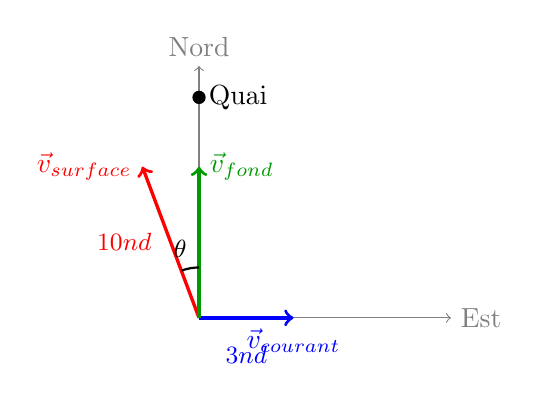
\begin{tikzpicture}[scale=0.8]
% Axes
\draw[gray, ->] (0,0) -- (4,0) node[right] {Est};
\draw[gray, ->] (0,0) -- (0,4) node[above] {Nord};
% Courant
\draw[very thick, blue, ->] (0,0) -- (1.5,0) node[below] {$\vec{v}_{courant}$};
\node[blue, below] at (0.75,-0.3) {\small $\SI{3}{nd}$};
% Vitesse surface (inclinée pour compenser)
\draw[very thick, red, ->] (0,0) -- (-0.9,2.4) node[left] {$\vec{v}_{surface}$};
\node[red, left] at (-0.6,1.2) {\small $\SI{10}{nd}$};
% Vitesse fond (résultante vers le nord)
\draw[very thick, green!60!black, ->] (0,0) -- (0,2.4) node[right] {$\vec{v}_{fond}$};
% Angle
\draw[thick] (0,0.8) arc (90:110:0.8);
\node at (-0.3,1.1) {\small $\theta$};
% Point d'arrivée
\fill (0,3.5) circle (3pt) node[right] {Quai};
\end{tikzpicture}
\end{center}

Pour que la vitesse fond soit dirig\'ee exactement vers le nord, le capitaine doit orienter son navire l\'eg\`erement vers l'ouest (cap correcteur).

\textbf{Angle de correction :}
\[ \sin\theta = \frac{v_{courant}}{v_{surface}} = \frac{3}{10} = 0,3 \quad \Rightarrow \quad \theta = 17{,}5° \text{ ouest du nord} \]

\textbf{Vitesse fond r\'esultante :}
\[ v_{fond} = v_{surface} \cos\theta = 10 \times \cos(17{,}5°) = \SI{9,5}{n\oe{}uds} \]
\end{exemple}

\begin{attention}
La vitesse relative est un concept vectoriel. En 2D, il faut d\'ecomposer les vitesses en composantes et les additionner vectoriellement. Ce sujet sera approfondi dans le cours de navigation.
\end{attention}
